\section{Introduction}
\label{sec:intro}

As the trend towards larger machine-learning models continue, from BERT~\cite{bert} with 340 million parameters, GPT-2~\cite{gpt-2} with 1.5 billion parameters, to GPT-3~\cite{gpt3} with 175 billion parameters, model training and inferencing have to be distributed. Moreover, as the computations become resource hungry, optimizing for even the last percentage can have huge benefits in terms of time, energy, and money savings~\cite{gpt3cost,strubell2019energy}.

In machine learning systems today, computation and communication are treated as independent abstractions implemented in different libraries. For instance, computation libraries, such as cuBLAS~\cite{cublas} and cuDNN~\cite{cudnn}, provide optimized tensor algebra operations, while communication libraries, like NVIDIA Collective Communications Library~\cite{nccl}, provide high-performance implementations of collective communication, such as \allreduce. Machine learning frameworks, such as PyTorch~\cite{pytorch}, call computation and communication kernels from these libraries. Thus, in machine learning applications built atop of such frameworks, the computation and communication operations are invoked separately.

While this separation allows independent optimization of computation and communication kernels, breaking this abstraction boundary can unlock new optimizations that are otherwise not feasible. These optimizations include the following. \emph{Interface} optimization eliminates a mismatch between the caller and the callee of an abstraction. For example, a machine learning model's parameters are stored in non-contiguous buffers, one buffer per layer and hence, need to copy all buffers into a single buffer before calling a collective communication like \allreduce. This copy can be avoided if the communication operation takes a list of arrays as input instead of requiring a single buffer. 
\emph{Fusion} optimization decreases memory bandwidth usage by generating a single kernel to perform multiple communication and computation operations. 
\emph{Reorder} optimization moves the computation before or after the communication, thereby either distributing the computation or enabling new fusion possibilities. 
Finally, \emph{overlapping} optimization orchestrates multiple computation and communication operations in a fine-grained manner to fully utilize both network and compute resources. We elaborate on this possibility below.  

\begin{figure}[t]
	\centering
  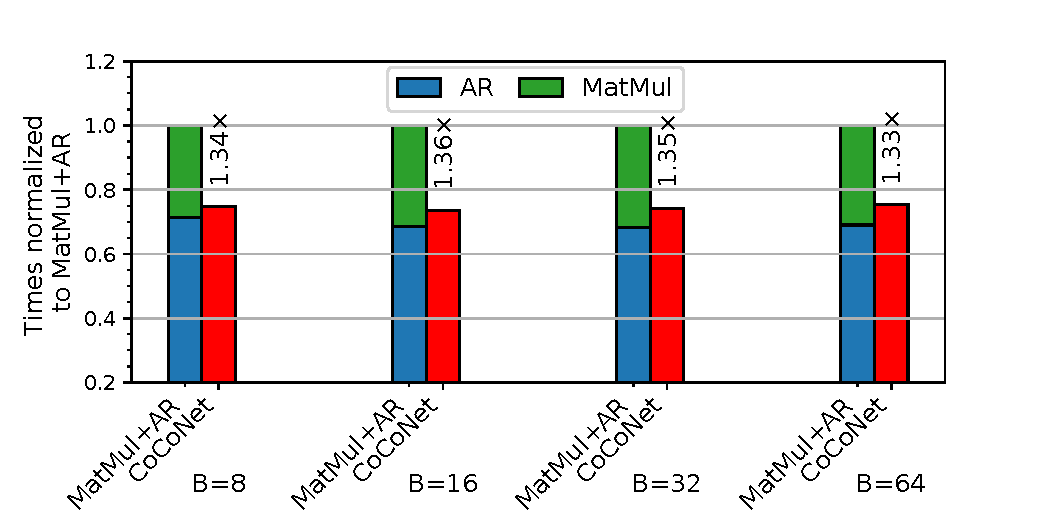
\includegraphics[width=\linewidth]{figures/matmul-overlap-with-streams-intro_small.pdf}
  \caption{Speedup of co-optimized overlapping over sequential MatMul and \allreduce (for model parallel GPT-2 Model input matrix of [B$\times$1024, 768] and weights of [768, 3072]) on 16 Tesla V100 GPUs.
  % The overlapping hides more than 80\% of GEMM behind \allreduce.
  \label{fig:matmul-overlap-intro}}
\end{figure}

In model parallelism, which is one of the distributed machine learning approaches, each layer is distributed across multiple GPUs \cite{megatronlm} and the computation for each layer consists of a matrix multiplication (MatMul) on each node followed by an \allreduce. 
The existing implementation of model parallelism calls individually optimized library functions for MatMul and \allreduce.
However, the implementation cannot utilize both network and computation resources simultaneously because the network is idle during MatMul.
We can completely utilize both network and computation resources simultaneously by overlapping the computation of MatMul with the communication of \allreduce in a fine-grained manner.
The idea is to slice the output into smaller chunks and start the \allreduce communication on a chunk as soon as the MatMul kernel has computed it.
To ensure minimum wait time for the \allreduce kernel, we need to schedule the MatMul kernel to compute chunks in the order the \allreduce kernel communicates them.
For instance, in the ring algorithm for \allreduce, the $n^{\text{th}}$ node sends the chunks to the next node in the 
order starting from the $n^{\text{th}}$ chunk. 
As such, the MatMul kernel on the $n^{\text{th}}$ node needs to generate the chunks in this order. 
Furthermore, we need to invoke only one MatMul kernel and \allreduce kernel to avoid the overhead of launching multiple kernels.
Figure~\ref{fig:matmul-overlap-intro} shows that this fine-grained overlapping of MatMul with \allreduce can hide 80\% of the execution time of MatMul and provides 1.36$\times$ speedup.

However, manually writing these optimizations for each scenario is unproductive, for example, the implementation of above overlapping optimization contains $\approx$2k lines of CUDA code.
Thus, in this paper, we show that by carefully designing a \emph{language} for expressing combinations of computation and communication the benefits of existing machine learning framework's abstraction can be maintained while simultaneously allowing a \emph{compiler} to apply powerful optimizations.
\begin{figure*}[t]
	\centering
  %	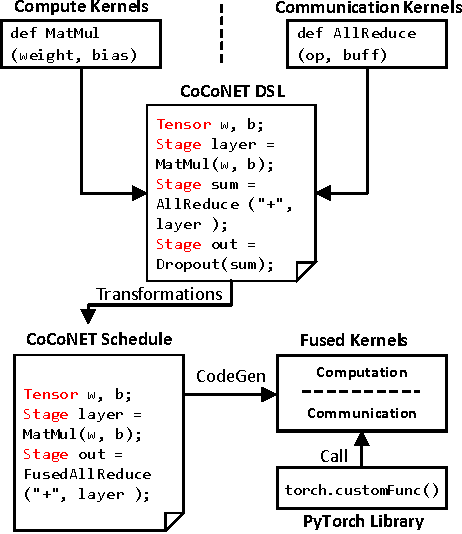
\includegraphics[width=.75\linewidth]{figures/overview-1column}
    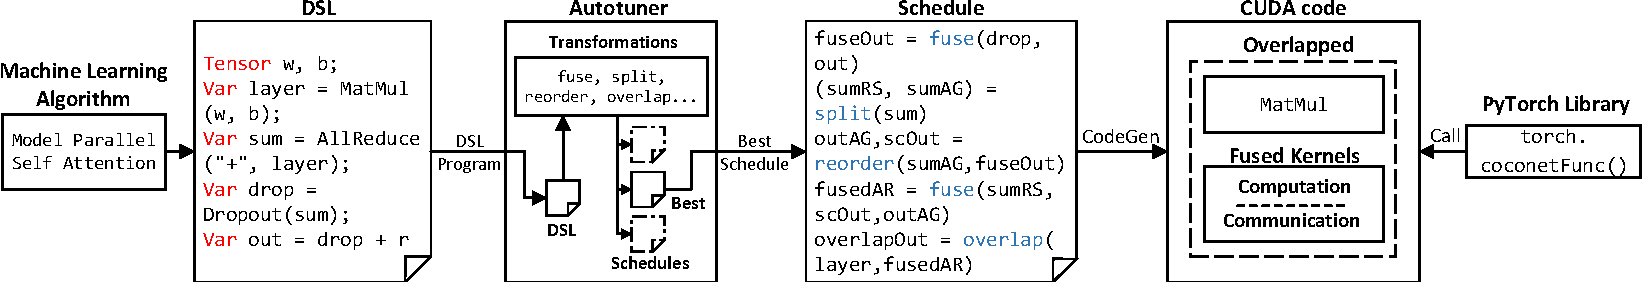
\includegraphics[width=\linewidth]{figures/overview-2}
    \caption{Overview of \tool's workflow. 
    First, a user expresses a machine learning algorithm in the DSL that contains both computation (MatMul) and communication (\allreduce).
    Then, the autotuner applies transformations to optimize the program while keeping the algorithm unchanged, such as fusing \allreduce and Dropout into FusedAllReduce and overlapping this with MatMul.
    Finally, \tool generates custom communication and computation code, which is available through PyTorch.}
    \label{fig:overview}
\end{figure*}
To this effect, we propose \tool\footnote{\tool stands for "{\bf \uline{Co}}mmunication and {\bf \uline{Co}}mputation optimization for neural {\bf \uline{Net}}works.}
for generating co-optimized custom computation and communication kernels.
Figure~\ref{fig:overview} presents the overview of \tool.
\tool includes a domain specific language (DSL) to express programs containing both computation and communication operations.
Inspired by Halide~\cite{halide}, \tool includes a \emph{scheduling} language 
to specify an execution schedule of the program using a set of transformations. 
\tool's \emph{autotuner} automatically applies these transformations to optimize a program by breaking the communication and computation boundary. 
Hence, \tool enables users to quickly generate optimized implementations for 
specific hardware, topology, and data sizes.
\tool's \emph{code generator} automatically generates high-performance computation and communication kernels from a program and its schedule.
%  and communication APIs and requires handoptimizing every workload, while the language level abstraction of \tool can automatically perform more optimizations on a program.
We used \tool to optimize data-parallel training, model-parallel inference, and pipeline-parallel inference. 
\tool generated kernels for the Adam~\cite{adam} and LAMB~\cite{lamb} optimizers speeds up
the training time of BERT models by upto 1.68$\times$ and can train BERT 3.9 Billion parameter models using only data parallelism, which is not possible with state of the arts.
\tool's kernels for model parallelism speeds up the inference in BERT 3.9 Billion and GPT-2 8.2 Billion parameter models by upto 1.51$\times$.
\tool's optimized pipeline parallelism kernels speeds up inference times in GPT-2 8.2 Billion and GPT-3 175 Billion parameter models by upto 1.77$\times$.
Our implementation of \tool is available at \url{https://github.com/parasailteam/coconet}.